\section{Progettazione Concettuale}
	
	\subsection{Strategia di Progetto}
		\emph{Top-down} per la realizzazione dello schema ad un adeguato livello di raffinamento. \emph{Inside-out} per la successiva correzione dello stesso.
		
		\emph{Questa sezione va ampliata e corretta}
		
	\subsection{Individuazione delle Entità Fondamentali}
		
		Dalle specifiche che abbiamo formulato risulta che uno dei punti fondamentali da affrontare è quello della memorizzazione dei preventivi emessi dall'attività.
		Ad ogni \emph{Prestazione} effettuata, corrisponde un \emph{Preventivo} precedentemente emesso.
		
		\vspace{0.5cm}
		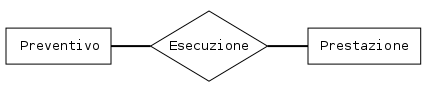
\includegraphics[width=11.5cm]{images/diagrams/preventivo_prestazione.png}
		\vspace{0.3cm}
		
		Il preventivo è formulato a fronte di un intervento richiesto da parte di un cliente alla propria autovettura, che esso riguardi una riparazione od una installazione. Si introducono quindi le entità \emph{Cliente} ed \emph{Autovettura}.
		
		\vspace{0.5cm}
		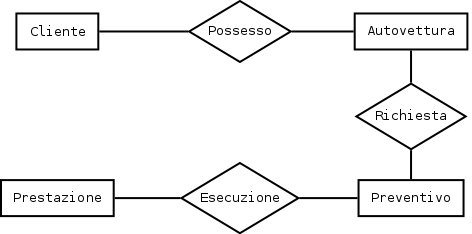
\includegraphics[width=11.5cm]{images/diagrams/cliente_prestazione.png}
		\vspace{0.3cm}
		
		Per la formulazione del preventivo, nonchè per il calcolo del costo finale dell'esecuzione della prestazione, sarà necessario conoscere i \emph{Componenti} previsti dall'operazione e quelli effettivamente utilizzati.
		
		\vspace{0.5cm}
		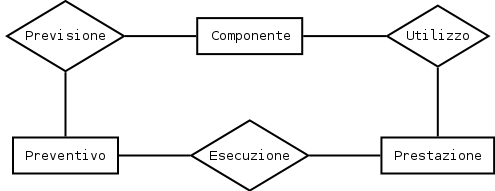
\includegraphics[width=11.5cm]{images/diagrams/componente_preventivo_prestazione.png}
		\vspace{0.3cm}
		
		